\documentclass[1p]{elsarticle_modified}
%\bibliographystyle{elsarticle-num}

%\usepackage[colorlinks]{hyperref}
%\usepackage{abbrmath_seonhwa} %\Abb, \Ascr, \Acal ,\Abf, \Afrak
\usepackage{amsfonts}
\usepackage{amssymb}
\usepackage{amsmath}
\usepackage{amsthm}
\usepackage{scalefnt}
\usepackage{amsbsy}
\usepackage{kotex}
\usepackage{caption}
\usepackage{subfig}
\usepackage{color}
\usepackage{graphicx}
\usepackage{xcolor} %% white, black, red, green, blue, cyan, magenta, yellow
\usepackage{float}
\usepackage{setspace}
\usepackage{hyperref}

\usepackage{tikz}
\usetikzlibrary{arrows}

\usepackage{multirow}
\usepackage{array} % fixed length table
\usepackage{hhline}

%%%%%%%%%%%%%%%%%%%%%
\makeatletter
\renewcommand*\env@matrix[1][\arraystretch]{%
	\edef\arraystretch{#1}%
	\hskip -\arraycolsep
	\let\@ifnextchar\new@ifnextchar
	\array{*\c@MaxMatrixCols c}}
\makeatother %https://tex.stackexchange.com/questions/14071/how-can-i-increase-the-line-spacing-in-a-matrix
%%%%%%%%%%%%%%%

\usepackage[normalem]{ulem}

\newcommand{\msout}[1]{\ifmmode\text{\sout{\ensuremath{#1}}}\else\sout{#1}\fi}
%SOURCE: \msout is \stkout macro in https://tex.stackexchange.com/questions/20609/strikeout-in-math-mode

\newcommand{\cancel}[1]{
	\ifmmode
	{\color{red}\msout{#1}}
	\else
	{\color{red}\sout{#1}}
	\fi
}

\newcommand{\add}[1]{
	{\color{blue}\uwave{#1}}
}

\newcommand{\replace}[2]{
	\ifmmode
	{\color{red}\msout{#1}}{\color{blue}\uwave{#2}}
	\else
	{\color{red}\sout{#1}}{\color{blue}\uwave{#2}}
	\fi
}

\newcommand{\Sol}{\mathcal{S}} %segment
\newcommand{\D}{D} %diagram
\newcommand{\A}{\mathcal{A}} %arc


%%%%%%%%%%%%%%%%%%%%%%%%%%%%%5 test

\def\sl{\operatorname{\textup{SL}}(2,\Cbb)}
\def\psl{\operatorname{\textup{PSL}}(2,\Cbb)}
\def\quan{\mkern 1mu \triangleright \mkern 1mu}

\theoremstyle{definition}
\newtheorem{thm}{Theorem}[section]
\newtheorem{prop}[thm]{Proposition}
\newtheorem{lem}[thm]{Lemma}
\newtheorem{ques}[thm]{Question}
\newtheorem{cor}[thm]{Corollary}
\newtheorem{defn}[thm]{Definition}
\newtheorem{exam}[thm]{Example}
\newtheorem{rmk}[thm]{Remark}
\newtheorem{alg}[thm]{Algorithm}

\newcommand{\I}{\sqrt{-1}}
\begin{document}

%\begin{frontmatter}
%
%\title{Boundary parabolic representations of knots up to 8 crossings}
%
%%% Group authors per affiliation:
%\author{Yunhi Cho} 
%\address{Department of Mathematics, University of Seoul, Seoul, Korea}
%\ead{yhcho@uos.ac.kr}
%
%
%\author{Seonhwa Kim} %\fnref{s_kim}}
%\address{Center for Geometry and Physics, Institute for Basic Science, Pohang, 37673, Korea}
%\ead{ryeona17@ibs.re.kr}
%
%\author{Hyuk Kim}
%\address{Department of Mathematical Sciences, Seoul National University, Seoul 08826, Korea}
%\ead{hyukkim@snu.ac.kr}
%
%\author{Seokbeom Yoon}
%\address{Department of Mathematical Sciences, Seoul National University, Seoul, 08826,  Korea}
%\ead{sbyoon15@snu.ac.kr}
%
%\begin{abstract}
%We find all boundary parabolic representation of knots up to 8 crossings.
%
%\end{abstract}
%\begin{keyword}
%    \MSC[2010] 57M25 
%\end{keyword}
%
%\end{frontmatter}

%\linenumbers
%\tableofcontents
%
\newcommand\colored[1]{\textcolor{white}{\rule[-0.35ex]{0.8em}{1.4ex}}\kern-0.8em\color{red} #1}%
%\newcommand\colored[1]{\textcolor{white}{ #1}\kern-2.17ex	\textcolor{white}{ #1}\kern-1.81ex	\textcolor{white}{ #1}\kern-2.15ex\color{red}#1	}

{\Large $\underline{12a_{1215}~(K12a_{1215})}$}

\setlength{\tabcolsep}{10pt}
\renewcommand{\arraystretch}{1.6}
\vspace{1cm}\begin{tabular}{m{100pt}>{\centering\arraybackslash}m{274pt}}
\multirow{5}{120pt}{
	\centering
	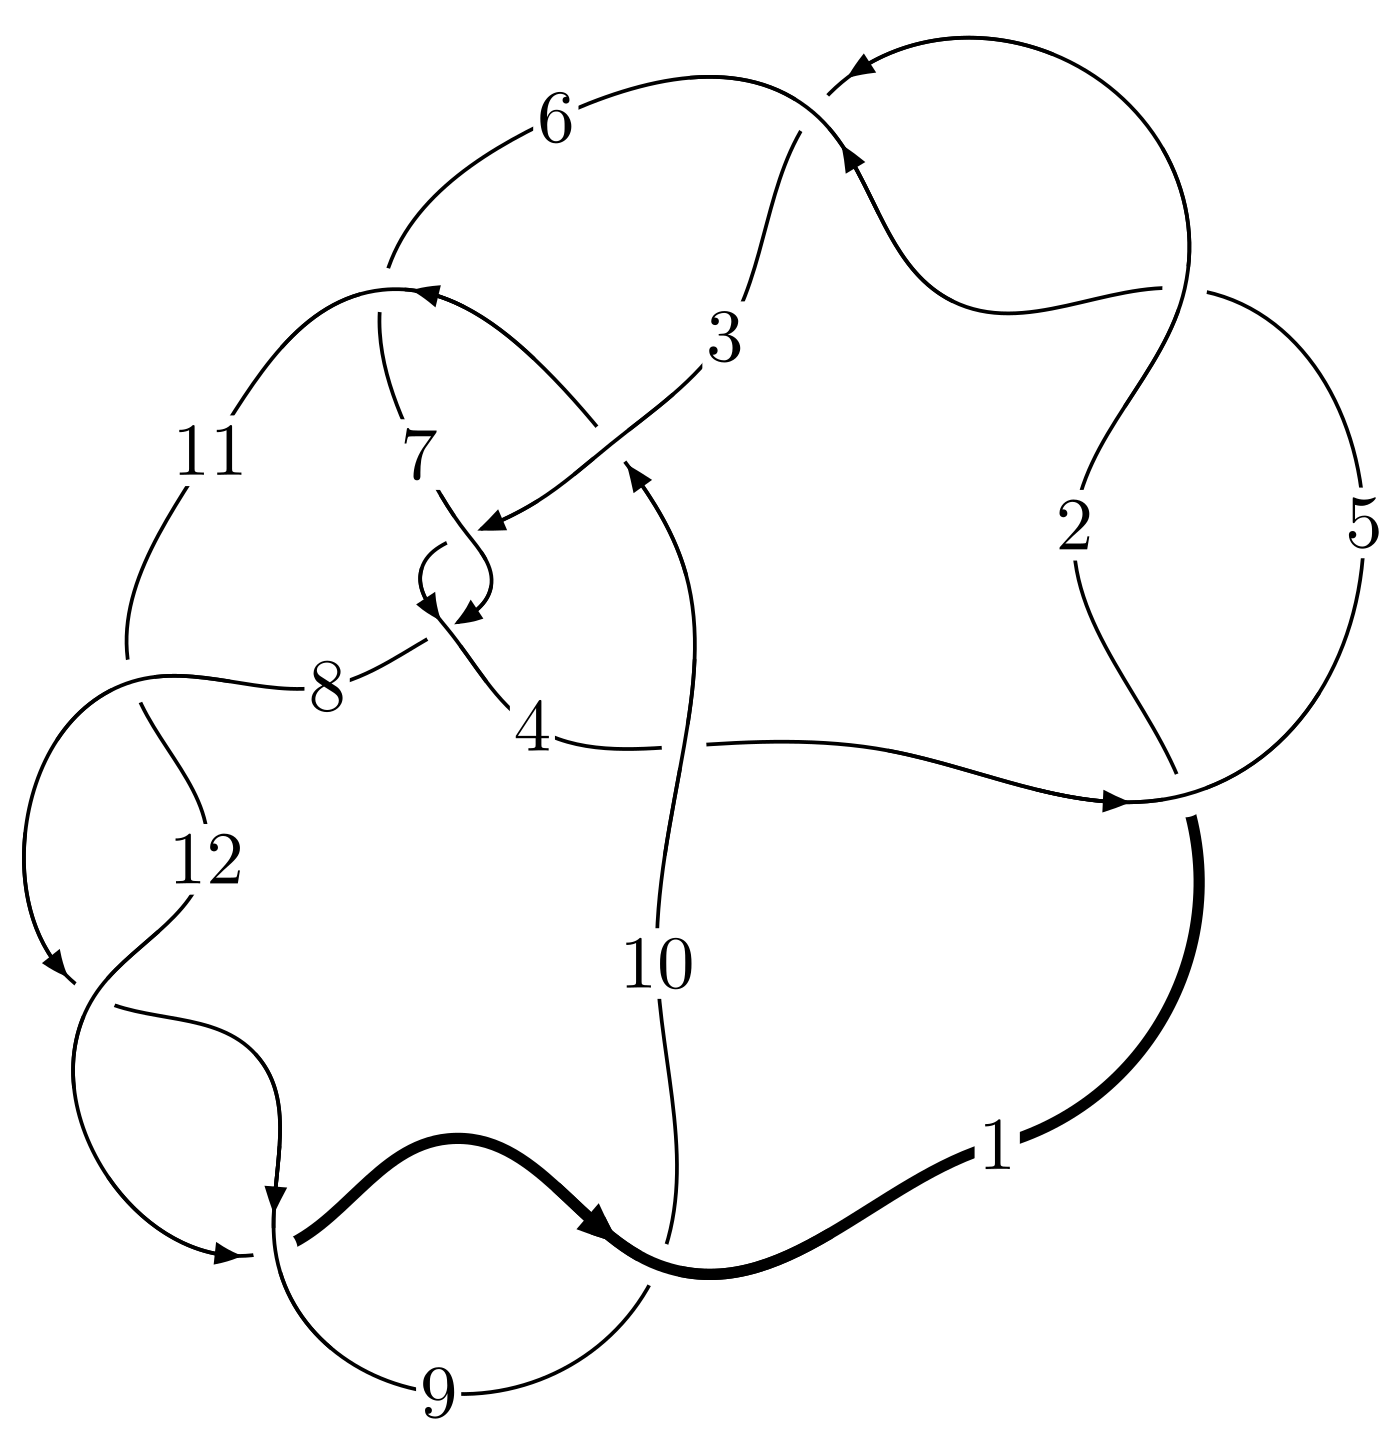
\includegraphics[width=112pt]{../../../GIT/diagram.site/Diagrams/png/2016_12a_1215.png}\\
\ \ \ A knot diagram\footnotemark}&
\allowdisplaybreaks
\textbf{Linearized knot diagam} \\
\cline{2-2}
 &
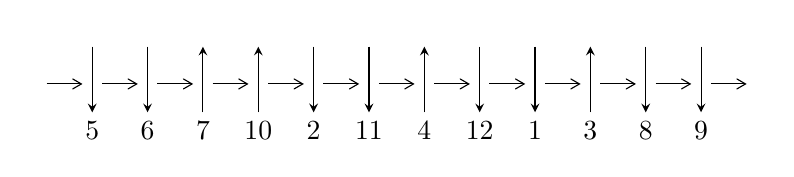
\begin{tikzpicture}[x=20pt, y=17pt]
	% nodes
	\node (C0) at (0, 0) {};
	\node (C1) at (1, 0) {};
	\node (C1U) at (1, +1) {};
	\node (C1D) at (1, -1) {5};

	\node (C2) at (2, 0) {};
	\node (C2U) at (2, +1) {};
	\node (C2D) at (2, -1) {6};

	\node (C3) at (3, 0) {};
	\node (C3U) at (3, +1) {};
	\node (C3D) at (3, -1) {7};

	\node (C4) at (4, 0) {};
	\node (C4U) at (4, +1) {};
	\node (C4D) at (4, -1) {10};

	\node (C5) at (5, 0) {};
	\node (C5U) at (5, +1) {};
	\node (C5D) at (5, -1) {2};

	\node (C6) at (6, 0) {};
	\node (C6U) at (6, +1) {};
	\node (C6D) at (6, -1) {11};

	\node (C7) at (7, 0) {};
	\node (C7U) at (7, +1) {};
	\node (C7D) at (7, -1) {4};

	\node (C8) at (8, 0) {};
	\node (C8U) at (8, +1) {};
	\node (C8D) at (8, -1) {12};

	\node (C9) at (9, 0) {};
	\node (C9U) at (9, +1) {};
	\node (C9D) at (9, -1) {1};

	\node (C10) at (10, 0) {};
	\node (C10U) at (10, +1) {};
	\node (C10D) at (10, -1) {3};

	\node (C11) at (11, 0) {};
	\node (C11U) at (11, +1) {};
	\node (C11D) at (11, -1) {8};

	\node (C12) at (12, 0) {};
	\node (C12U) at (12, +1) {};
	\node (C12D) at (12, -1) {9};
	\node (C13) at (13, 0) {};

	% arrows
	\draw[->,>={angle 60}]
	(C0) edge (C1) (C1) edge (C2) (C2) edge (C3) (C3) edge (C4) (C4) edge (C5) (C5) edge (C6) (C6) edge (C7) (C7) edge (C8) (C8) edge (C9) (C9) edge (C10) (C10) edge (C11) (C11) edge (C12) (C12) edge (C13) ;	\draw[->,>=stealth]
	(C1U) edge (C1D) (C2U) edge (C2D) (C3D) edge (C3U) (C4D) edge (C4U) (C5U) edge (C5D) (C6U) edge (C6D) (C7D) edge (C7U) (C8U) edge (C8D) (C9U) edge (C9D) (C10D) edge (C10U) (C11U) edge (C11D) (C12U) edge (C12D) ;
	\end{tikzpicture} \\
\hhline{~~} \\& 
\textbf{Solving Sequence} \\ \cline{2-2} 
 &
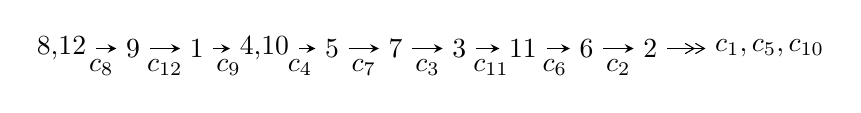
\begin{tikzpicture}[x=23pt, y=7pt]
	% node
	\node (A0) at (-1/8, 0) {8,12};
	\node (A1) at (1, 0) {9};
	\node (A2) at (2, 0) {1};
	\node (A3) at (49/16, 0) {4,10};
	\node (A4) at (33/8, 0) {5};
	\node (A5) at (41/8, 0) {7};
	\node (A6) at (49/8, 0) {3};
	\node (A7) at (57/8, 0) {11};
	\node (A8) at (65/8, 0) {6};
	\node (A9) at (73/8, 0) {2};
	\node (C1) at (1/2, -1) {$c_{8}$};
	\node (C2) at (3/2, -1) {$c_{12}$};
	\node (C3) at (5/2, -1) {$c_{9}$};
	\node (C4) at (29/8, -1) {$c_{4}$};
	\node (C5) at (37/8, -1) {$c_{7}$};
	\node (C6) at (45/8, -1) {$c_{3}$};
	\node (C7) at (53/8, -1) {$c_{11}$};
	\node (C8) at (61/8, -1) {$c_{6}$};
	\node (C9) at (69/8, -1) {$c_{2}$};
	\node (A10) at (11, 0) {$c_{1},c_{5},c_{10}$};

	% edge
	\draw[->,>=stealth]	
	(A0) edge (A1) (A1) edge (A2) (A2) edge (A3) (A3) edge (A4) (A4) edge (A5) (A5) edge (A6) (A6) edge (A7) (A7) edge (A8) (A8) edge (A9) ;
	\draw[->>,>={angle 60}]	
	(A9) edge (A10);
\end{tikzpicture} \\ 

\end{tabular} \\

\footnotetext{
The image of knot diagram is generated by the software ``\textbf{Draw programme}" developed by Andrew Bartholomew(\url{http://www.layer8.co.uk/maths/draw/index.htm\#Running-draw}), where we modified some parts for our purpose(\url{https://github.com/CATsTAILs/LinksPainter}).
}\phantom \\ \newline 
\centering \textbf{Ideals for irreducible components\footnotemark of $X_{\text{par}}$} 
 
\begin{align*}
I^u_{1}&=\langle 
8.53148\times10^{61} u^{60}-2.63560\times10^{62} u^{59}+\cdots+2.09325\times10^{62} b-3.25181\times10^{62},\\
\phantom{I^u_{1}}&\phantom{= \langle  }-2.51402\times10^{63} u^{60}+8.62823\times10^{63} u^{59}+\cdots+2.09325\times10^{62} a+4.65225\times10^{63},\;u^{61}-4 u^{60}+\cdots-2 u+1\rangle \\
I^u_{2}&=\langle 
b+1,\;a^2+2 a-1,\;u-1\rangle \\
I^u_{3}&=\langle 
b-1,\;a-1,\;u-1\rangle \\
\\
\end{align*}
\raggedright * 3 irreducible components of $\dim_{\mathbb{C}}=0$, with total 64 representations.\\
\footnotetext{All coefficients of polynomials are rational numbers. But the coefficients are sometimes approximated in decimal forms when there is not enough margin.}
\newpage
\renewcommand{\arraystretch}{1}
\centering \section*{I. $I^u_{1}= \langle 8.53\times10^{61} u^{60}-2.64\times10^{62} u^{59}+\cdots+2.09\times10^{62} b-3.25\times10^{62},\;-2.51\times10^{63} u^{60}+8.63\times10^{63} u^{59}+\cdots+2.09\times10^{62} a+4.65\times10^{63},\;u^{61}-4 u^{60}+\cdots-2 u+1 \rangle$}
\flushleft \textbf{(i) Arc colorings}\\
\begin{tabular}{m{7pt} m{180pt} m{7pt} m{180pt} }
\flushright $a_{8}=$&$\begin{pmatrix}1\\0\end{pmatrix}$ \\
\flushright $a_{12}=$&$\begin{pmatrix}0\\u\end{pmatrix}$ \\
\flushright $a_{9}=$&$\begin{pmatrix}1\\u^2\end{pmatrix}$ \\
\flushright $a_{1}=$&$\begin{pmatrix}- u\\- u^3+u\end{pmatrix}$ \\
\flushright $a_{4}=$&$\begin{pmatrix}12.0101 u^{60}-41.2193 u^{59}+\cdots+70.6756 u-22.2250\\-0.407570 u^{60}+1.25909 u^{59}+\cdots+1.20398 u+1.55347\end{pmatrix}$ \\
\flushright $a_{10}=$&$\begin{pmatrix}- u^2+1\\- u^4+2 u^2\end{pmatrix}$ \\
\flushright $a_{5}=$&$\begin{pmatrix}7.23475 u^{60}-25.7491 u^{59}+\cdots+71.7086 u-14.2434\\-5.32045 u^{60}+17.2364 u^{59}+\cdots-2.23417 u+8.89499\end{pmatrix}$ \\
\flushright $a_{7}=$&$\begin{pmatrix}12.4952 u^{60}-42.3313 u^{59}+\cdots+65.7255 u-22.9269\\-0.0236838 u^{60}+0.0968098 u^{59}+\cdots+2.88901 u+0.876791\end{pmatrix}$ \\
\flushright $a_{3}=$&$\begin{pmatrix}-1.23183 u^{60}+2.22698 u^{59}+\cdots+10.3657 u+2.23332\\-1.82728 u^{60}+4.13641 u^{59}+\cdots-3.93849 u+1.46849\end{pmatrix}$ \\
\flushright $a_{11}=$&$\begin{pmatrix}u\\u\end{pmatrix}$ \\
\flushright $a_{6}=$&$\begin{pmatrix}7.14430 u^{60}-25.0978 u^{59}+\cdots+62.9492 u-15.2793\\-5.37461 u^{60}+17.3303 u^{59}+\cdots+0.112788 u+8.52436\end{pmatrix}$ \\
\flushright $a_{2}=$&$\begin{pmatrix}-8.78259 u^{60}+27.8143 u^{59}+\cdots+85.7450 u+9.78144\\5.73116 u^{60}-20.6175 u^{59}+\cdots+6.59694 u-9.06352\end{pmatrix}$\\&\end{tabular}
\flushleft \textbf{(ii) Obstruction class $= -1$}\\~\\
\flushleft \textbf{(iii) Cusp Shapes $= -112.270 u^{60}+381.730 u^{59}+\cdots-78.0643 u+180.153$}\\~\\
\newpage\renewcommand{\arraystretch}{1}
\flushleft \textbf{(iv) u-Polynomials at the component}\newline \\
\begin{tabular}{m{50pt}|m{274pt}}
Crossings & \hspace{64pt}u-Polynomials at each crossing \\
\hline $$\begin{aligned}c_{1},c_{2},c_{5}\end{aligned}$$&$\begin{aligned}
&u^{61}+5 u^{60}+\cdots-6 u+2
\end{aligned}$\\
\hline $$\begin{aligned}c_{3},c_{7}\end{aligned}$$&$\begin{aligned}
&u^{61}-2 u^{60}+\cdots-18 u-1
\end{aligned}$\\
\hline $$\begin{aligned}c_{4}\end{aligned}$$&$\begin{aligned}
&u^{61}+14 u^{60}+\cdots-20506 u+253751
\end{aligned}$\\
\hline $$\begin{aligned}c_{6}\end{aligned}$$&$\begin{aligned}
&u^{61}-16 u^{60}+\cdots-298 u-71
\end{aligned}$\\
\hline $$\begin{aligned}c_{8},c_{9},c_{11}\\c_{12}\end{aligned}$$&$\begin{aligned}
&u^{61}+4 u^{60}+\cdots-2 u-1
\end{aligned}$\\
\hline $$\begin{aligned}c_{10}\end{aligned}$$&$\begin{aligned}
&u^{61}+2 u^{60}+\cdots+2 u-1
\end{aligned}$\\
\hline
\end{tabular}\\~\\
\newpage\renewcommand{\arraystretch}{1}
\flushleft \textbf{(v) Riley Polynomials at the component}\newline \\
\begin{tabular}{m{50pt}|m{274pt}}
Crossings & \hspace{64pt}Riley Polynomials at each crossing \\
\hline $$\begin{aligned}c_{1},c_{2},c_{5}\end{aligned}$$&$\begin{aligned}
&y^{61}-67 y^{60}+\cdots+68 y-4
\end{aligned}$\\
\hline $$\begin{aligned}c_{3},c_{7}\end{aligned}$$&$\begin{aligned}
&y^{61}-34 y^{60}+\cdots+206 y-1
\end{aligned}$\\
\hline $$\begin{aligned}c_{4}\end{aligned}$$&$\begin{aligned}
&y^{61}-654 y^{60}+\cdots-751092018078 y-64389570001
\end{aligned}$\\
\hline $$\begin{aligned}c_{6}\end{aligned}$$&$\begin{aligned}
&y^{61}-674 y^{60}+\cdots+204818 y-5041
\end{aligned}$\\
\hline $$\begin{aligned}c_{8},c_{9},c_{11}\\c_{12}\end{aligned}$$&$\begin{aligned}
&y^{61}-74 y^{60}+\cdots-98 y-1
\end{aligned}$\\
\hline $$\begin{aligned}c_{10}\end{aligned}$$&$\begin{aligned}
&y^{61}+2 y^{60}+\cdots+102 y-1
\end{aligned}$\\
\hline
\end{tabular}\\~\\
\newpage\flushleft \textbf{(vi) Complex Volumes and Cusp Shapes}
$$\begin{array}{c|c|c}  
\text{Solutions to }I^u_{1}& \I (\text{vol} + \sqrt{-1}CS) & \text{Cusp shape}\\
 \hline 
\begin{aligned}
u &= \phantom{-}0.746185 + 0.718329 I \\
a &= \phantom{-}0.782846 + 0.678292 I \\
b &= -0.677631 + 0.453749 I\end{aligned}
 & -7.75122 - 2.10321 I & \phantom{-0.000000 } 0 \\ \hline\begin{aligned}
u &= \phantom{-}0.746185 - 0.718329 I \\
a &= \phantom{-}0.782846 - 0.678292 I \\
b &= -0.677631 - 0.453749 I\end{aligned}
 & -7.75122 + 2.10321 I & \phantom{-0.000000 } 0 \\ \hline\begin{aligned}
u &= -0.967076 + 0.398497 I \\
a &= -0.312053 + 0.858947 I \\
b &= -0.128262 + 0.982641 I\end{aligned}
 & -10.05700 + 6.18751 I & \phantom{-0.000000 } 0 \\ \hline\begin{aligned}
u &= -0.967076 - 0.398497 I \\
a &= -0.312053 - 0.858947 I \\
b &= -0.128262 - 0.982641 I\end{aligned}
 & -10.05700 - 6.18751 I & \phantom{-0.000000 } 0 \\ \hline\begin{aligned}
u &= -0.814186 + 0.491497 I \\
a &= -0.27925 + 1.52542 I \\
b &= \phantom{-}1.238410 + 0.560509 I\end{aligned}
 & \phantom{-}0.54223 + 8.36059 I & \phantom{-0.000000 } 0 \\ \hline\begin{aligned}
u &= -0.814186 - 0.491497 I \\
a &= -0.27925 - 1.52542 I \\
b &= \phantom{-}1.238410 - 0.560509 I\end{aligned}
 & \phantom{-}0.54223 - 8.36059 I & \phantom{-0.000000 } 0 \\ \hline\begin{aligned}
u &= \phantom{-}1.07507\phantom{ +0.000000I} \\
a &= \phantom{-}1.21685\phantom{ +0.000000I} \\
b &= \phantom{-}0.0908214\phantom{ +0.000000I}\end{aligned}
 & -6.55025\phantom{ +0.000000I} & \phantom{-0.000000 } 0 \\ \hline\begin{aligned}
u &= -0.919328 + 0.600137 I \\
a &= \phantom{-}0.37668 - 1.39219 I \\
b &= -1.252060 - 0.562320 I\end{aligned}
 & -6.64410 + 11.69040 I & \phantom{-0.000000 } 0 \\ \hline\begin{aligned}
u &= -0.919328 - 0.600137 I \\
a &= \phantom{-}0.37668 + 1.39219 I \\
b &= -1.252060 + 0.562320 I\end{aligned}
 & -6.64410 - 11.69040 I & \phantom{-0.000000 } 0 \\ \hline\begin{aligned}
u &= \phantom{-}1.035030 + 0.370907 I \\
a &= \phantom{-}0.389492 - 0.314417 I \\
b &= \phantom{-}0.923451 + 0.227131 I\end{aligned}
 & -0.586497 + 0.638281 I & \phantom{-0.000000 } 0\\
 \hline 
 \end{array}$$\newpage$$\begin{array}{c|c|c}  
\text{Solutions to }I^u_{1}& \I (\text{vol} + \sqrt{-1}CS) & \text{Cusp shape}\\
 \hline 
\begin{aligned}
u &= \phantom{-}1.035030 - 0.370907 I \\
a &= \phantom{-}0.389492 + 0.314417 I \\
b &= \phantom{-}0.923451 - 0.227131 I\end{aligned}
 & -0.586497 - 0.638281 I & \phantom{-0.000000 } 0 \\ \hline\begin{aligned}
u &= -0.022074 + 0.884978 I \\
a &= \phantom{-}0.760719 + 0.081071 I \\
b &= -1.116060 + 0.470898 I\end{aligned}
 & -3.89787 - 6.79256 I & \phantom{-0.000000 } 0 \\ \hline\begin{aligned}
u &= -0.022074 - 0.884978 I \\
a &= \phantom{-}0.760719 - 0.081071 I \\
b &= -1.116060 - 0.470898 I\end{aligned}
 & -3.89787 + 6.79256 I & \phantom{-0.000000 } 0 \\ \hline\begin{aligned}
u &= -0.784824 + 0.190256 I \\
a &= \phantom{-}0.337219 - 1.157560 I \\
b &= \phantom{-}0.146848 - 1.059540 I\end{aligned}
 & -2.79892 + 2.75782 I & -12.5719 - 8.9610 I \\ \hline\begin{aligned}
u &= -0.784824 - 0.190256 I \\
a &= \phantom{-}0.337219 + 1.157560 I \\
b &= \phantom{-}0.146848 + 1.059540 I\end{aligned}
 & -2.79892 - 2.75782 I & -12.5719 + 8.9610 I \\ \hline\begin{aligned}
u &= \phantom{-}0.609495 + 0.503426 I \\
a &= -0.901420 - 0.967851 I \\
b &= \phantom{-}0.770857 - 0.254010 I\end{aligned}
 & -0.88592 - 1.76991 I & -10.70286 + 7.10949 I \\ \hline\begin{aligned}
u &= \phantom{-}0.609495 - 0.503426 I \\
a &= -0.901420 + 0.967851 I \\
b &= \phantom{-}0.770857 + 0.254010 I\end{aligned}
 & -0.88592 + 1.76991 I & -10.70286 - 7.10949 I \\ \hline\begin{aligned}
u &= -0.701647 + 0.311220 I \\
a &= -0.02710 - 1.68276 I \\
b &= -1.217220 - 0.602617 I\end{aligned}
 & \phantom{-}1.19274 + 3.49963 I & -4.99930 - 7.32299 I \\ \hline\begin{aligned}
u &= -0.701647 - 0.311220 I \\
a &= -0.02710 + 1.68276 I \\
b &= -1.217220 + 0.602617 I\end{aligned}
 & \phantom{-}1.19274 - 3.49963 I & -4.99930 + 7.32299 I \\ \hline\begin{aligned}
u &= -0.760212 + 0.073205 I \\
a &= \phantom{-}0.457673 - 0.810260 I \\
b &= \phantom{-}1.46334 - 0.51937 I\end{aligned}
 & -5.23021 + 0.94975 I & -19.2405 - 6.6283 I\\
 \hline 
 \end{array}$$\newpage$$\begin{array}{c|c|c}  
\text{Solutions to }I^u_{1}& \I (\text{vol} + \sqrt{-1}CS) & \text{Cusp shape}\\
 \hline 
\begin{aligned}
u &= -0.760212 - 0.073205 I \\
a &= \phantom{-}0.457673 + 0.810260 I \\
b &= \phantom{-}1.46334 + 0.51937 I\end{aligned}
 & -5.23021 - 0.94975 I & -19.2405 + 6.6283 I \\ \hline\begin{aligned}
u &= \phantom{-}1.086370 + 0.613746 I \\
a &= -0.145908 + 0.115784 I \\
b &= -0.881548 - 0.426034 I\end{aligned}
 & -7.18543 + 1.66168 I & \phantom{-0.000000 } 0 \\ \hline\begin{aligned}
u &= \phantom{-}1.086370 - 0.613746 I \\
a &= -0.145908 - 0.115784 I \\
b &= -0.881548 + 0.426034 I\end{aligned}
 & -7.18543 - 1.66168 I & \phantom{-0.000000 } 0 \\ \hline\begin{aligned}
u &= \phantom{-}0.740049\phantom{ +0.000000I} \\
a &= -0.465551\phantom{ +0.000000I} \\
b &= \phantom{-}0.111226\phantom{ +0.000000I}\end{aligned}
 & -1.28803\phantom{ +0.000000I} & -7.85780\phantom{ +0.000000I} \\ \hline\begin{aligned}
u &= \phantom{-}0.217246 + 0.690863 I \\
a &= \phantom{-}0.585924 + 0.057283 I \\
b &= -0.219547 - 0.599860 I\end{aligned}
 & -6.43015 - 2.58923 I & -10.03195 + 2.41589 I \\ \hline\begin{aligned}
u &= \phantom{-}0.217246 - 0.690863 I \\
a &= \phantom{-}0.585924 - 0.057283 I \\
b &= -0.219547 + 0.599860 I\end{aligned}
 & -6.43015 + 2.58923 I & -10.03195 - 2.41589 I \\ \hline\begin{aligned}
u &= -0.077144 + 0.695385 I \\
a &= -0.802000 + 0.155188 I \\
b &= \phantom{-}1.138390 - 0.392051 I\end{aligned}
 & \phantom{-}2.78020 - 4.38394 I & -1.53700 + 6.52121 I \\ \hline\begin{aligned}
u &= -0.077144 - 0.695385 I \\
a &= -0.802000 - 0.155188 I \\
b &= \phantom{-}1.138390 + 0.392051 I\end{aligned}
 & \phantom{-}2.78020 + 4.38394 I & -1.53700 - 6.52121 I \\ \hline\begin{aligned}
u &= \phantom{-}0.623061 + 0.152291 I \\
a &= -0.39384 + 3.45519 I \\
b &= -0.923865 + 0.057323 I\end{aligned}
 & \phantom{-}0.488805 - 0.376151 I & \phantom{-}9.8390 - 11.6732 I \\ \hline\begin{aligned}
u &= \phantom{-}0.623061 - 0.152291 I \\
a &= -0.39384 - 3.45519 I \\
b &= -0.923865 - 0.057323 I\end{aligned}
 & \phantom{-}0.488805 + 0.376151 I & \phantom{-}9.8390 + 11.6732 I\\
 \hline 
 \end{array}$$\newpage$$\begin{array}{c|c|c}  
\text{Solutions to }I^u_{1}& \I (\text{vol} + \sqrt{-1}CS) & \text{Cusp shape}\\
 \hline 
\begin{aligned}
u &= \phantom{-}0.624285\phantom{ +0.000000I} \\
a &= -36.9272\phantom{ +0.000000I} \\
b &= \phantom{-}1.01546\phantom{ +0.000000I}\end{aligned}
 & -4.28785\phantom{ +0.000000I} & \phantom{-}381.270\phantom{ +0.000000I} \\ \hline\begin{aligned}
u &= \phantom{-}1.38099\phantom{ +0.000000I} \\
a &= -0.737085\phantom{ +0.000000I} \\
b &= -1.32091\phantom{ +0.000000I}\end{aligned}
 & -1.75297\phantom{ +0.000000I} & \phantom{-0.000000 } 0 \\ \hline\begin{aligned}
u &= -0.146537 + 0.414207 I \\
a &= \phantom{-}0.599805 - 0.923128 I \\
b &= -1.184330 + 0.269776 I\end{aligned}
 & \phantom{-}2.80305 - 0.88629 I & \phantom{-}0.82315 - 2.43589 I \\ \hline\begin{aligned}
u &= -0.146537 - 0.414207 I \\
a &= \phantom{-}0.599805 + 0.923128 I \\
b &= -1.184330 - 0.269776 I\end{aligned}
 & \phantom{-}2.80305 + 0.88629 I & \phantom{-}0.82315 + 2.43589 I \\ \hline\begin{aligned}
u &= -1.60938 + 0.03982 I \\
a &= -0.35124 - 1.78283 I \\
b &= -0.934436 - 0.284454 I\end{aligned}
 & -7.29629 + 1.06963 I & \phantom{-0.000000 } 0 \\ \hline\begin{aligned}
u &= -1.60938 - 0.03982 I \\
a &= -0.35124 + 1.78283 I \\
b &= -0.934436 + 0.284454 I\end{aligned}
 & -7.29629 - 1.06963 I & \phantom{-0.000000 } 0 \\ \hline\begin{aligned}
u &= -1.61455 + 0.13274 I \\
a &= \phantom{-}0.040334 + 1.272930 I \\
b &= \phantom{-}0.970713 + 0.461820 I\end{aligned}
 & -8.57121 + 4.07733 I & \phantom{-0.000000 } 0 \\ \hline\begin{aligned}
u &= -1.61455 - 0.13274 I \\
a &= \phantom{-}0.040334 - 1.272930 I \\
b &= \phantom{-}0.970713 - 0.461820 I\end{aligned}
 & -8.57121 - 4.07733 I & \phantom{-0.000000 } 0 \\ \hline\begin{aligned}
u &= -1.62277\phantom{ +0.000000I} \\
a &= -5.90882\phantom{ +0.000000I} \\
b &= \phantom{-}1.08441\phantom{ +0.000000I}\end{aligned}
 & -12.2377\phantom{ +0.000000I} & \phantom{-0.000000 } 0 \\ \hline\begin{aligned}
u &= \phantom{-}1.62759 + 0.06997 I \\
a &= -0.77048 + 1.60057 I \\
b &= -1.33629 + 0.86263 I\end{aligned}
 & -6.89593 - 4.83384 I & \phantom{-0.000000 } 0\\
 \hline 
 \end{array}$$\newpage$$\begin{array}{c|c|c}  
\text{Solutions to }I^u_{1}& \I (\text{vol} + \sqrt{-1}CS) & \text{Cusp shape}\\
 \hline 
\begin{aligned}
u &= \phantom{-}1.62759 - 0.06997 I \\
a &= -0.77048 - 1.60057 I \\
b &= -1.33629 - 0.86263 I\end{aligned}
 & -6.89593 + 4.83384 I & \phantom{-0.000000 } 0 \\ \hline\begin{aligned}
u &= \phantom{-}1.64847 + 0.04117 I \\
a &= \phantom{-}0.30494 + 1.78899 I \\
b &= \phantom{-}0.22966 + 1.43807 I\end{aligned}
 & -11.30720 - 3.57722 I & \phantom{-0.000000 } 0 \\ \hline\begin{aligned}
u &= \phantom{-}1.64847 - 0.04117 I \\
a &= \phantom{-}0.30494 - 1.78899 I \\
b &= \phantom{-}0.22966 - 1.43807 I\end{aligned}
 & -11.30720 + 3.57722 I & \phantom{-0.000000 } 0 \\ \hline\begin{aligned}
u &= \phantom{-}1.64947 + 0.01439 I \\
a &= \phantom{-}1.12320 + 0.98345 I \\
b &= \phantom{-}1.74629 + 0.70290 I\end{aligned}
 & -13.72070 - 1.24651 I & \phantom{-0.000000 } 0 \\ \hline\begin{aligned}
u &= \phantom{-}1.64947 - 0.01439 I \\
a &= \phantom{-}1.12320 - 0.98345 I \\
b &= \phantom{-}1.74629 - 0.70290 I\end{aligned}
 & -13.72070 + 1.24651 I & \phantom{-0.000000 } 0 \\ \hline\begin{aligned}
u &= \phantom{-}1.65001 + 0.13394 I \\
a &= \phantom{-}0.50978 - 1.60334 I \\
b &= \phantom{-}1.31764 - 0.70879 I\end{aligned}
 & -7.91826 - 10.72950 I & \phantom{-0.000000 } 0 \\ \hline\begin{aligned}
u &= \phantom{-}1.65001 - 0.13394 I \\
a &= \phantom{-}0.50978 + 1.60334 I \\
b &= \phantom{-}1.31764 + 0.70879 I\end{aligned}
 & -7.91826 + 10.72950 I & \phantom{-0.000000 } 0 \\ \hline\begin{aligned}
u &= \phantom{-}0.123537 + 0.319863 I \\
a &= -1.021060 - 0.481385 I \\
b &= \phantom{-}0.014084 + 0.425125 I\end{aligned}
 & -0.233943 - 0.995944 I & -4.40045 + 6.40501 I \\ \hline\begin{aligned}
u &= \phantom{-}0.123537 - 0.319863 I \\
a &= -1.021060 + 0.481385 I \\
b &= \phantom{-}0.014084 - 0.425125 I\end{aligned}
 & -0.233943 + 0.995944 I & -4.40045 - 6.40501 I \\ \hline\begin{aligned}
u &= -1.65674 + 0.03555 I \\
a &= \phantom{-}0.362387 - 0.621120 I \\
b &= \phantom{-}0.449534 - 0.418699 I\end{aligned}
 & -9.99487 + 0.25967 I & \phantom{-0.000000 } 0\\
 \hline 
 \end{array}$$\newpage$$\begin{array}{c|c|c}  
\text{Solutions to }I^u_{1}& \I (\text{vol} + \sqrt{-1}CS) & \text{Cusp shape}\\
 \hline 
\begin{aligned}
u &= -1.65674 - 0.03555 I \\
a &= \phantom{-}0.362387 + 0.621120 I \\
b &= \phantom{-}0.449534 + 0.418699 I\end{aligned}
 & -9.99487 - 0.25967 I & \phantom{-0.000000 } 0 \\ \hline\begin{aligned}
u &= -1.67432 + 0.22629 I \\
a &= \phantom{-}0.020974 - 1.105390 I \\
b &= -0.981377 - 0.576312 I\end{aligned}
 & -16.0070 + 5.8071 I & \phantom{-0.000000 } 0 \\ \hline\begin{aligned}
u &= -1.67432 - 0.22629 I \\
a &= \phantom{-}0.020974 + 1.105390 I \\
b &= -0.981377 + 0.576312 I\end{aligned}
 & -16.0070 - 5.8071 I & \phantom{-0.000000 } 0 \\ \hline\begin{aligned}
u &= \phantom{-}1.68740 + 0.17394 I \\
a &= -0.34603 + 1.54557 I \\
b &= -1.34464 + 0.64636 I\end{aligned}
 & -15.5798 - 14.7360 I & \phantom{-0.000000 } 0 \\ \hline\begin{aligned}
u &= \phantom{-}1.68740 - 0.17394 I \\
a &= -0.34603 - 1.54557 I \\
b &= -1.34464 - 0.64636 I\end{aligned}
 & -15.5798 + 14.7360 I & \phantom{-0.000000 } 0 \\ \hline\begin{aligned}
u &= \phantom{-}1.69400 + 0.10712 I \\
a &= -0.32490 - 1.47775 I \\
b &= -0.139744 - 1.234560 I\end{aligned}
 & -19.3348 - 8.1899 I & \phantom{-0.000000 } 0 \\ \hline\begin{aligned}
u &= \phantom{-}1.69400 - 0.10712 I \\
a &= -0.32490 + 1.47775 I \\
b &= -0.139744 + 1.234560 I\end{aligned}
 & -19.3348 + 8.1899 I & \phantom{-0.000000 } 0 \\ \hline\begin{aligned}
u &= -1.73658 + 0.10391 I \\
a &= -0.204374 + 0.738826 I \\
b &= -0.512503 + 0.660988 I\end{aligned}
 & -17.3526 + 1.0261 I & \phantom{-0.000000 } 0 \\ \hline\begin{aligned}
u &= -1.73658 - 0.10391 I \\
a &= -0.204374 - 0.738826 I \\
b &= -0.512503 - 0.660988 I\end{aligned}
 & -17.3526 - 1.0261 I & \phantom{-0.000000 } 0 \\ \hline\begin{aligned}
u &= -0.0120702 + 0.1398260 I \\
a &= -1.36141 + 8.95063 I \\
b &= \phantom{-}0.949803 + 0.197306 I\end{aligned}
 & -3.17091 - 0.11856 I & -2.06650 - 1.49742 I\\
 \hline 
 \end{array}$$\newpage$$\begin{array}{c|c|c}  
\text{Solutions to }I^u_{1}& \I (\text{vol} + \sqrt{-1}CS) & \text{Cusp shape}\\
 \hline 
\begin{aligned}
u &= -0.0120702 - 0.1398260 I \\
a &= -1.36141 - 8.95063 I \\
b &= \phantom{-}0.949803 - 0.197306 I\end{aligned}
 & -3.17091 + 0.11856 I & -2.06650 + 1.49742 I\\
 \hline 
 \end{array}$$\newpage\newpage\renewcommand{\arraystretch}{1}
\centering \section*{II. $I^u_{2}= \langle b+1,\;a^2+2 a-1,\;u-1 \rangle$}
\flushleft \textbf{(i) Arc colorings}\\
\begin{tabular}{m{7pt} m{180pt} m{7pt} m{180pt} }
\flushright $a_{8}=$&$\begin{pmatrix}1\\0\end{pmatrix}$ \\
\flushright $a_{12}=$&$\begin{pmatrix}0\\1\end{pmatrix}$ \\
\flushright $a_{9}=$&$\begin{pmatrix}1\\1\end{pmatrix}$ \\
\flushright $a_{1}=$&$\begin{pmatrix}-1\\0\end{pmatrix}$ \\
\flushright $a_{4}=$&$\begin{pmatrix}a\\-1\end{pmatrix}$ \\
\flushright $a_{10}=$&$\begin{pmatrix}0\\1\end{pmatrix}$ \\
\flushright $a_{5}=$&$\begin{pmatrix}a\\- a-1\end{pmatrix}$ \\
\flushright $a_{7}=$&$\begin{pmatrix}- a+1\\1\end{pmatrix}$ \\
\flushright $a_{3}=$&$\begin{pmatrix}1\\0\end{pmatrix}$ \\
\flushright $a_{11}=$&$\begin{pmatrix}1\\1\end{pmatrix}$ \\
\flushright $a_{6}=$&$\begin{pmatrix}1\\a+1\end{pmatrix}$ \\
\flushright $a_{2}=$&$\begin{pmatrix}- a\\-2\end{pmatrix}$\\&\end{tabular}
\flushleft \textbf{(ii) Obstruction class $= 1$}\\~\\
\flushleft \textbf{(iii) Cusp Shapes $= -8$}\\~\\
\newpage\renewcommand{\arraystretch}{1}
\flushleft \textbf{(iv) u-Polynomials at the component}\newline \\
\begin{tabular}{m{50pt}|m{274pt}}
Crossings & \hspace{64pt}u-Polynomials at each crossing \\
\hline $$\begin{aligned}c_{1},c_{2},c_{5}\end{aligned}$$&$\begin{aligned}
&u^2-2
\end{aligned}$\\
\hline $$\begin{aligned}c_{3},c_{8},c_{9}\end{aligned}$$&$\begin{aligned}
&(u-1)^2
\end{aligned}$\\
\hline $$\begin{aligned}c_{4}\end{aligned}$$&$\begin{aligned}
&u^2+2 u-1
\end{aligned}$\\
\hline $$\begin{aligned}c_{6}\end{aligned}$$&$\begin{aligned}
&u^2-2 u-1
\end{aligned}$\\
\hline $$\begin{aligned}c_{7},c_{10},c_{11}\\c_{12}\end{aligned}$$&$\begin{aligned}
&(u+1)^2
\end{aligned}$\\
\hline
\end{tabular}\\~\\
\newpage\renewcommand{\arraystretch}{1}
\flushleft \textbf{(v) Riley Polynomials at the component}\newline \\
\begin{tabular}{m{50pt}|m{274pt}}
Crossings & \hspace{64pt}Riley Polynomials at each crossing \\
\hline $$\begin{aligned}c_{1},c_{2},c_{5}\end{aligned}$$&$\begin{aligned}
&(y-2)^2
\end{aligned}$\\
\hline $$\begin{aligned}c_{3},c_{7},c_{8}\\c_{9},c_{10},c_{11}\\c_{12}\end{aligned}$$&$\begin{aligned}
&(y-1)^2
\end{aligned}$\\
\hline $$\begin{aligned}c_{4},c_{6}\end{aligned}$$&$\begin{aligned}
&y^2-6 y+1
\end{aligned}$\\
\hline
\end{tabular}\\~\\
\newpage\flushleft \textbf{(vi) Complex Volumes and Cusp Shapes}
$$\begin{array}{c|c|c}  
\text{Solutions to }I^u_{2}& \I (\text{vol} + \sqrt{-1}CS) & \text{Cusp shape}\\
 \hline 
\begin{aligned}
u &= \phantom{-}1.00000\phantom{ +0.000000I} \\
a &= \phantom{-}0.414214\phantom{ +0.000000I} \\
b &= -1.00000\phantom{ +0.000000I}\end{aligned}
 & -4.93480\phantom{ +0.000000I} & -8.00000\phantom{ +0.000000I} \\ \hline\begin{aligned}
u &= \phantom{-}1.00000\phantom{ +0.000000I} \\
a &= -2.41421\phantom{ +0.000000I} \\
b &= -1.00000\phantom{ +0.000000I}\end{aligned}
 & -4.93480\phantom{ +0.000000I} & -8.00000\phantom{ +0.000000I}\\
 \hline 
 \end{array}$$\newpage\newpage\renewcommand{\arraystretch}{1}
\centering \section*{III. $I^u_{3}= \langle b-1,\;a-1,\;u-1 \rangle$}
\flushleft \textbf{(i) Arc colorings}\\
\begin{tabular}{m{7pt} m{180pt} m{7pt} m{180pt} }
\flushright $a_{8}=$&$\begin{pmatrix}1\\0\end{pmatrix}$ \\
\flushright $a_{12}=$&$\begin{pmatrix}0\\1\end{pmatrix}$ \\
\flushright $a_{9}=$&$\begin{pmatrix}1\\1\end{pmatrix}$ \\
\flushright $a_{1}=$&$\begin{pmatrix}-1\\0\end{pmatrix}$ \\
\flushright $a_{4}=$&$\begin{pmatrix}1\\1\end{pmatrix}$ \\
\flushright $a_{10}=$&$\begin{pmatrix}0\\1\end{pmatrix}$ \\
\flushright $a_{5}=$&$\begin{pmatrix}1\\0\end{pmatrix}$ \\
\flushright $a_{7}=$&$\begin{pmatrix}2\\1\end{pmatrix}$ \\
\flushright $a_{3}=$&$\begin{pmatrix}-1\\0\end{pmatrix}$ \\
\flushright $a_{11}=$&$\begin{pmatrix}1\\1\end{pmatrix}$ \\
\flushright $a_{6}=$&$\begin{pmatrix}1\\0\end{pmatrix}$ \\
\flushright $a_{2}=$&$\begin{pmatrix}-1\\0\end{pmatrix}$\\&\end{tabular}
\flushleft \textbf{(ii) Obstruction class $= 1$}\\~\\
\flushleft \textbf{(iii) Cusp Shapes $= 0$}\\~\\
\newpage\renewcommand{\arraystretch}{1}
\flushleft \textbf{(iv) u-Polynomials at the component}\newline \\
\begin{tabular}{m{50pt}|m{274pt}}
Crossings & \hspace{64pt}u-Polynomials at each crossing \\
\hline $$\begin{aligned}c_{1},c_{2},c_{5}\end{aligned}$$&$\begin{aligned}
&u
\end{aligned}$\\
\hline $$\begin{aligned}c_{3},c_{11},c_{12}\end{aligned}$$&$\begin{aligned}
&u+1
\end{aligned}$\\
\hline $$\begin{aligned}c_{4},c_{6},c_{7}\\c_{8},c_{9},c_{10}\end{aligned}$$&$\begin{aligned}
&u-1
\end{aligned}$\\
\hline
\end{tabular}\\~\\
\newpage\renewcommand{\arraystretch}{1}
\flushleft \textbf{(v) Riley Polynomials at the component}\newline \\
\begin{tabular}{m{50pt}|m{274pt}}
Crossings & \hspace{64pt}Riley Polynomials at each crossing \\
\hline $$\begin{aligned}c_{1},c_{2},c_{5}\end{aligned}$$&$\begin{aligned}
&y
\end{aligned}$\\
\hline $$\begin{aligned}c_{3},c_{4},c_{6}\\c_{7},c_{8},c_{9}\\c_{10},c_{11},c_{12}\end{aligned}$$&$\begin{aligned}
&y-1
\end{aligned}$\\
\hline
\end{tabular}\\~\\
\newpage\flushleft \textbf{(vi) Complex Volumes and Cusp Shapes}
$$\begin{array}{c|c|c}  
\text{Solutions to }I^u_{3}& \I (\text{vol} + \sqrt{-1}CS) & \text{Cusp shape}\\
 \hline 
\begin{aligned}
u &= \phantom{-}1.00000\phantom{ +0.000000I} \\
a &= \phantom{-}1.00000\phantom{ +0.000000I} \\
b &= \phantom{-}1.00000\phantom{ +0.000000I}\end{aligned}
 & \phantom{-0.000000 } 0 & \phantom{-0.000000 } 0\\
 \hline 
 \end{array}$$\newpage
\newpage\renewcommand{\arraystretch}{1}
\centering \section*{ IV. u-Polynomials}
\begin{tabular}{m{50pt}|m{274pt}}
Crossings & \hspace{64pt}u-Polynomials at each crossing \\
\hline $$\begin{aligned}c_{1},c_{2},c_{5}\end{aligned}$$&$\begin{aligned}
&u(u^2-2)(u^{61}+5 u^{60}+\cdots-6 u+2)
\end{aligned}$\\
\hline $$\begin{aligned}c_{3}\end{aligned}$$&$\begin{aligned}
&((u-1)^2)(u+1)(u^{61}-2 u^{60}+\cdots-18 u-1)
\end{aligned}$\\
\hline $$\begin{aligned}c_{4}\end{aligned}$$&$\begin{aligned}
&(u-1)(u^2+2 u-1)(u^{61}+14 u^{60}+\cdots-20506 u+253751)
\end{aligned}$\\
\hline $$\begin{aligned}c_{6}\end{aligned}$$&$\begin{aligned}
&(u-1)(u^2-2 u-1)(u^{61}-16 u^{60}+\cdots-298 u-71)
\end{aligned}$\\
\hline $$\begin{aligned}c_{7}\end{aligned}$$&$\begin{aligned}
&(u-1)(u+1)^2(u^{61}-2 u^{60}+\cdots-18 u-1)
\end{aligned}$\\
\hline $$\begin{aligned}c_{8},c_{9}\end{aligned}$$&$\begin{aligned}
&((u-1)^3)(u^{61}+4 u^{60}+\cdots-2 u-1)
\end{aligned}$\\
\hline $$\begin{aligned}c_{10}\end{aligned}$$&$\begin{aligned}
&(u-1)(u+1)^2(u^{61}+2 u^{60}+\cdots+2 u-1)
\end{aligned}$\\
\hline $$\begin{aligned}c_{11},c_{12}\end{aligned}$$&$\begin{aligned}
&((u+1)^3)(u^{61}+4 u^{60}+\cdots-2 u-1)
\end{aligned}$\\
\hline
\end{tabular}\newpage\renewcommand{\arraystretch}{1}
\centering \section*{ V. Riley Polynomials}
\begin{tabular}{m{50pt}|m{274pt}}
Crossings & \hspace{64pt}Riley Polynomials at each crossing \\
\hline $$\begin{aligned}c_{1},c_{2},c_{5}\end{aligned}$$&$\begin{aligned}
&y(y-2)^2(y^{61}-67 y^{60}+\cdots+68 y-4)
\end{aligned}$\\
\hline $$\begin{aligned}c_{3},c_{7}\end{aligned}$$&$\begin{aligned}
&((y-1)^3)(y^{61}-34 y^{60}+\cdots+206 y-1)
\end{aligned}$\\
\hline $$\begin{aligned}c_{4}\end{aligned}$$&$\begin{aligned}
&(y-1)(y^2-6 y+1)\\
&\cdot(y^{61}-654 y^{60}+\cdots-751092018078 y-64389570001)
\end{aligned}$\\
\hline $$\begin{aligned}c_{6}\end{aligned}$$&$\begin{aligned}
&(y-1)(y^2-6 y+1)(y^{61}-674 y^{60}+\cdots+204818 y-5041)
\end{aligned}$\\
\hline $$\begin{aligned}c_{8},c_{9},c_{11}\\c_{12}\end{aligned}$$&$\begin{aligned}
&((y-1)^3)(y^{61}-74 y^{60}+\cdots-98 y-1)
\end{aligned}$\\
\hline $$\begin{aligned}c_{10}\end{aligned}$$&$\begin{aligned}
&((y-1)^3)(y^{61}+2 y^{60}+\cdots+102 y-1)
\end{aligned}$\\
\hline
\end{tabular}
\vskip 2pc
\end{document}